%!TEX root = ../report.tex
\chapter{Tools and Methods}
\label{cha:tools_and_methods}
The theory behind Sentiment Analysis and sentiment lexicon creation involves a large range of concepts within the fields of machine learning, natural language processing and statistics. The natural language processing part of Sentiment Analysis is concerned with analysing and highlighting features in text, while the machine learning part is concerned with structuring and learning patterns from the features extracted. Statistical methods are used as an integral part of machine learning as well as playing a central role in the creation of sentiment lexica. In this chapter, the most relevant concepts within the aforementioned fields are detailed, before the different tools and datasets used throughout development are described. 

\section{Central Concepts in Sentiment Analysis}
\label{sec:background_nlp}

\subsection*{Bag-of-Words}
The Bag-of-Words model is a commonly used model when classifying text documents or sentences. The model, as indicated by its name, represents the text as a ``bag of words''. The \textit{bag} contains all used words and keeps track of the specific word frequencies without any structure or order. The model it creates can be used directly as a feature vector in a machine learning classifier.

\subsection*{$n$-gram}
An $n$-gram could be a single word or character appearing in a document, or a collection of words or characters appearing consecutively in a document. These two types of $n$-grams are called \textit{Word n-grams} and \textit{Character n-grams}. The $n$ in $n$-gram stands for the number of consecutive words or characters to look at.  In the \textit{Bag-of-Words} model presented above, \textit{Word n-grams} with $n = 1$ are used and the model is only looking at single independent words. With $n>1$ the same principle can be applied by treating $n$ consecutive tokens as if they were a single. 

\subsection*{Part-of-Speech Tagging}
\ac{pos} tagging is the process of tagging each word in a text with its lexical category. The different categories are the different parts of speech, such as noun, verb and adjective. This categorization depends on the actual definition of the words themselves and the contexts they are in (relationships with adjacent words or other words in the text or sentence). Most \ac{pos} taggers are trained on treebanks in the newswire domain, where most of the training data is formal and well written text. The performance of these taggers commonly degrades on out-of-domain data. As stated by \cite{Gimpel11}, data such as tweets bring additional difficulties like misspellings, slang and a limited number of characters, and therefore a specialized \ac{pos} tagger for tweets is needed. 

\subsection*{Negation}
Negation in natural language is used to change the sentiment polarity of a word, a phrase or an entire sentence. Words that on their own appear to have a positive sentiment can in fact have a negative sentiment in a negated context. For example, \textit{``I am happy''} has positive sentiment, while \textit{``I am not happy''} has negative sentiment. However, negation does not always reverse the polarity entirely, sometimes negation only changes the magnitude of the polarity. For example, \textit{``I am very happy''} has high positive sentiment, while \textit{``I am not very happy''} is still positive, but not as much. \\

To negate a phrase, words called negators are used. These are also known as \textit{negation-cues} or \textit{negation-signals} and comprise words such as \textit{not}, \textit{won't}, \textit{can't} and \textit{doesn't}. Detecting these negators in a sentence is fundamental when trying to say something about the overall sentiment of a sentence. 

\subsection*{Sentiment Lexicon}
Lexicon based approaches are based around the idea of calculating the overall sentiment of a text as a function of the sentiment values of the words or phrases in it. The lexicon can be created manually by assigning a score to each word/phrase, or automatically. One example of automatic lexicon creation is to start with some manually classified seed words and assign a similar value to words that commonly appear together with the seed words.

\subsection*{Word Clusters}
\label{sec:background_cluster}
The word clustering technique is an attempt to reduce the data sparsity of natural languages. Instead of considering each misspelling, different grammatical forms of a word or synonyms as own and unique words, words are translated using a dictionary to a cluster ID. A common technique to generate word clusters is to use Brown clustering, by \cite{Brown92}, which is based on Hidden Markov Models. After the translation, the cluster IDs can be used in a simple Bag-of-Words model.

\section{Measures}

\subsection{Pointwise Mutual Information}
\label{sec:pointwise_mutual_information}
\ac{pmi} is an association measure quantifying the amount of information shared between two or more events. According to \cite{fano1961transmission}, given two events $x$ and $y$ with joint probability $P(x, y)$ and individual probabilities $P(x)$ and $P(y)$, their mutual information $I(x, y)$ is defined to be:

\begin{equation}
\label{eq:pmi}
    I(x, y) = log_2 \frac{P(x, y)}{P(x)P(y)}
\end{equation}

The mutual information is the comparison of the probabilities of observing the events $x$ and $y$ \textit{together} and the probabilities of observing them \textit{individually}. If there is an association between the two events $x$ and $y$, then their joint probability will be higher than the product of the individual probabilities, that is, $P(x, y) > P(x)P(y)$. Then, the chance of observing $x$ becomes greater if $y$ has already been observed. If the events are independent, the joint probability will be equal to the product of the individual probabilities $P(x, y) = P(x)P(y)$, which leads to $I(x, y) = 0$, meaning that there are no interesting relationship between the events. \\

The \ac{pmi} measure as apposed to the mutual information (MI) measure, uses Equation~\ref{eq:pmi} on single events and not on a series of possible events. When using the \ac{pmi} measure, $x$ and $y$ are single and specific events, whereas $x$ and $y$ can take on multiple values using MI.

\subsection*{PMI $n$-grams}
One of the applications of the \ac{pmi} measure is finding collocations and associations between words. This is achieved by counting single word occurrences and co-occurrences in a corpus to determine the probabilities $P(x, y)$ and $P(x)$, before using Equation~\ref{eq:pmi} on each pair of words. The word pairs with high \ac{pmi} values are the words that together form common phrases or collocations in the chosen corpus. Using the \ac{pmi} measure in this manner was first introduced by \cite{Church90} and has since become a common method for finding meaningful word $n$-grams. The \ac{pmi} measure can also be used on $n$-grams with $n>2$ using the \ac{pmi}-chain rule:

\begin{equation}
\begin{aligned}
    PMI(x, yz) &= PMI(x,y) + PMI(x, z|y)\\
        &= log_2 \frac{P(x, y)}{P(x)P(y)} + log_2 \frac{P(x, z|y)}{P(x|y)P(z|y)}\\
        &= log_2 \frac{P(x, yz)}{P(x)P(yz)}
\end{aligned}
\end{equation}


\subsection{Term Frequency---Inverse Document Frequency}
\label{sec:background_tfidf}
The \ac{tfidf} is a numerical statistic that provides the bag-of-words model with information about word importance. The word importance comes in the form of a weighting-scheme over all words where words with high weights provide more information than words with low weights. The actual weight each word is given is a combination of the Term Frequency ($TF$), Document Frequency ($DF$) and the Inverse Document Frequency ($IDF$) as conceived by \cite{SparckJones72}. Term Frequency is the number of times a given term appears in a given document, Document Frequency is the number of documents that contain a given term, and Inverse Document Frequency is a measure of how much information a given term provides in a set of $N$ documents. The \ac{tfidf} weight of a term within a document is calculated as follows, where $t$ is a term appearing in document $d$: \\

\begin{equation}
    \text{TF-IDF}\left(t,\, d\right) = \text{TF}\left(t,\, d\right)\cdot \text{IDF}\left(t\right)
\end{equation}

\begin{equation}
    \text{IDF}\left(t\right) = \log\frac{N}{\text{DF}\left(t\right)}
\end{equation}

As stated by \cite{Manning08}, a word will thus get a high weight if it appears often in a small amount of documents and a lower weight if it occurs few times in a document or many times across all documents. If a word occurs many times across all documents, it will get the smallest possible weight. Common words not providing much information, such as: `the', `a' and `is', will therefore tend to get low weights.

\subsection{Levenshtein Distance}
\label{sec:levenshtein}
Levenshtein distance or edit distance, is a similarity metric proposed by \cite{levenshtein66} used to measure the difference between two strings. The edit distance is determined by how many INSERT, DELETE or SUBSTITUTE operations that are needed to transform one string into another. The process of calculating the distance is shown in Algorithm~\ref{alg:levenshtein}.  

\begin{algorithm}
	\DontPrintSemicolon
    \caption{Levenshtein Distance Algorithm}
    \label{alg:levenshtein}
    \KwIn{\textbf{char} $a_{1..m}$, \textbf{char} $b_{1..n}$}
    \KwOut{Edit distance between two strings, $distance \in \mathbb{N}$}
    
 	$d_{i,0}=i$, $\forall i$\;
	$d_{0,j}=j$, $\forall j$\;
    
    \For{$i \gets 1$ \textbf{to} $m$}{
    	\For{$j \gets 1$ \textbf{to} $n$}{
    		\eIf{$a_i = b_j$}{
            	$cost := 0$\;
            }{
            	$cost := 1$\;
            }
            $d_{i,j} :=$ \textbf{min}(\;
            	\hspace*{1.5em}$d_{i-1, j} + 1$,		\tcp*{deletion}
                \hspace*{1.5em}$d_{i, j-1} + 1$,		\tcp*{insertion}
                \hspace*{1.5em}$d_{i-1, j-1} + cost$)	\tcp*{substitution}
    	}
    }
   \textbf{return} $d_{m, n}$
\end{algorithm}

\subsection{Cosine Similarity}
\label{sec:cosine_similarity}
Cosine similarity is a measure used to calculate the similarity between two vectors, based on the cosine of the angle between them. If used in a positive space the resulting similarity is bounded within the range [0,1]. An angle of 0\degree{} between two vectors, will yield a perfect similarity of 1, while an angle of 90\degree{} yields a similarity of 0. The cosine similarity is calculated as follows:

\begin{equation}
    Cosine Similarity(A, B) = \frac{\sum\limits_{i=1}^{n}A_i B_i}{\sqrt{\sum\limits_{i=1}^{n}A_i^2} \sqrt{\sum\limits_{i=1}^{n}B_i^2}}
\end{equation}

\noindent where $A_i$ and $B_i$ represent the different dimension values of the vectors $A$ and $B$ respectively.


\subsection{Pearson's Correlation}
\label{sec:pearson_correlation}
The Pearson's Correlation or Pearson product-moment-correlation coefficient is a measure used to determine the correlation between two variables and was developed by \cite{Pearson253}. If the two variables are perfectly positively correlated, the measure yields a correlation value of 1, whilst two variables that are perfectly negatively correlated gets a correlation value of -1. For two points with no correlation, a correlation value of 0 is given. The correlation $r_{xy}$ between two vectors $x$ and $y$ is calculated using the following formula:


\begin{equation}
    r_{xy} = \frac{\sum\limits_{i=1}^{n}(x_i-\bar{x})(y_i-\bar{y})}{\sqrt{\sum\limits_{i=1}^{n}(x_i-\bar{x})^2}\sqrt{\sum\limits_{i=1}^{n}(y_i-\bar{y})^2}}
\end{equation}
where $n$ is the size of the vectors $x$ and $y$, while $\bar{x}$ and $\bar{y}$ are their mean values. \\

Pearson Correlation can also be used when normalizing matrices. Then the correlation between all row and column pairs are calculated before the values are normalized between -1 and 1. The complete normalization process is captured in the following formula:

\begin{equation}
\label{eq:pearson_normalization}
    w_{ab}^{'}=\frac{Tw_{ab}-\sum_{j}w_{aj}\cdot\sum_{i}w_{ib}}{(\sum_{j}w_{aj}\cdot(T-\sum_{j}w_{aj})\cdot\sum_{i}w_{ib}\cdot(T-\sum_{i}w_{ib}))^\frac{1}{2}}
\end{equation}
where $T$ is the sum of all elements in the matrix.


\section{Lexicon Creation}
\subsection{PMI Lexicon}
\label{sec:pmi_lexicon}
An application of the \ac{pmi} measure is in creating sentiment lexica. \cite{turneylittman2002} proposed a method where the sentimental orientation of a word could be calculated from the \ac{pmi} value of a word $w$ in a positive context $PMI(w, positive)$ and the same word in a negative context $PMI(w, negative)$ using the equation:

\begin{equation}
\label{eq:sentiment_score}
    Sentiment Score(w) = PMI(w, positive) - PMI(w, negative)
\end{equation}

Here $PMI(w, positive)$ and $PMI(w, negative)$ are calculated using:

\begin{equation}
\label{eq:pmi_orientation}
    PMI(w, orientation) = log_2 \frac{freq(w, orientation) \cdot N}{freq(w) \cdot freq(orientation)},
\end{equation}

\noindent where $freq(w)$ is the number of times term $w$ appears in a document, while $N$ is total number of terms in the document. Equation~\ref{eq:sentiment_score} can then be rewritten to:

\begin{equation}
\label{eq:sentiment_score_final}
    Sentiment Score(w) = log_2 \frac{freq(w, positive) \cdot freq(negative)}{freq(w, negative) \cdot freq(positive)}
\end{equation}

Determining whether a word is in a positive or negative context can be done in different ways. \citeauthor{turneylittman2002} use a method based on a seed set of positive and negative words and decide the context of a word based on whether or not the word is found in close proximity to either a positive or negative seed word. \cite{MohammadKZ2013} similarly use a seed set, but instead of containing positive and negative words, the seed set contains positive and negative hashtags and emoticons. In addition, complete sentences, or tweets in this case, were labeled in contrast to the single word labeling suggested by \citeauthor{turneylittman2002}. The labeling was based on the occurrence of a seed set hashtag or emoticon within each tweet. Complete documents that are already labeled, such as user reviews or hand labeled sentences, for instance, can use Equation~\ref{eq:sentiment_score} directly.


\subsection{Label Propagation Algorithm}
\label{sec:label_propagation_algorithm}
The Label Propagation Algorithm (LPA) is a graph propagation algorithm proposed by \cite{Zhu02learningfrom} and is used to label unlabeled entities, to detect clusters or communities within a dataset. The algorithm can either be initialized with all nodes having an initial label or with only a few nodes being labeled. The algorithm is iterative, where in each iteration the nodes are selected in random order and given the label most common among the neighboring nodes. When no node changes label during an iteration the algorithm finishes. When only some of the nodes are initially labeled, those nodes commonly reset their label after each iteration.\\

Determining which nodes are neighboring each other or the weights of the edges between the nodes can be done in different ways. The edges represent the similarity or another relationship between the entities, and depending on this relationship an appropriate measure is chosen to determine the relational strength among all of the entities. An edge is commonly created between two nodes, making them neighboring nodes, if their relational strength is above a predefined threshold. Some of the most common measures used to calculate relational strengths are cosine similarity, co-occurrence statistics and \ac{pmi}. \\

\subsection*{LPA Lexicon}
One application of the Label Propagation Algorithm is to infer a sentiment lexicon. This can be done by initializing nodes representing seed words with their sentiment value, while the rest of the nodes, representing the candidate lexicon entries, remain unlabeled. The sentiment values of the seed words are then propagated through the graph setting the sentiment value of each candidate entry node to the weighted sum of its neighbors sentiment values. When convergence has been achieved the algorithm is terminated, and each candidate entry has been given its final sentiment value. The process is shown in Algorithm~\ref{alg:label_propagation}. \\

\begin{algorithm}
	\DontPrintSemicolon
    \caption{Label Propagation Algorithm}
    \label{alg:label_propagation}
    \KwIn{$G=(V,E)$, $w_{ij}\in[0,1]$, $P$, $N$}
    \KwOut{Sentiment Lexicon, $pol \in \mathbb{R}^{|V|}$}
    
    $pol_i = 0$, $\forall i$\;
	$pol_i = 1.0$, $\forall v_i \in P$\;
    $pol_i = -1.0$, $\forall v_i \in N$\;

	\For{$t \gets 1$ \textbf{to} $T$}{
		$pol_i = \frac{\sum_{(v_i, v_j) \in E} w_{ij} \cdot pol_j}{\sum_{(v_i, v_j) \in E} w_{ij}}$, $\forall v_i \in V$\;
        $pol_i = 1.0$, $\forall v_i \in P$\tcp*{Reset positive seed words}
    	$pol_i = -1.0$, $\forall v_i \in N$\tcp*{Reset negative seed words}
    }
\end{algorithm}

A problem highlighted by \cite{Velikovich2010} when using LPA to create a sentiment lexicon, is what is called the reinforcement effect. Because the sentiment value of each node is calculated as the weighted sum of its neighbors, each node could be influenced by the same seed node multiple times. In graphs with many dense subgraphs and occurrences of erroneous edges, the number of paths from seed words could get very high, resulting in an amplified flow of sentiment. This could lead to words that are supposed to get similar sentiment values end up with very different sentiment values. Additionally, \citeauthor{Velikovich2010} discovered that negative phrases appeared more densely connected, resulting in a lexicon highly skewered towards negative entries. The effect is illustrated in Figure~\ref{fig:label_propagation}.

\begin{figure}[t]
    \centering
    \begin{subfigure}[b]{1.0\textwidth}
        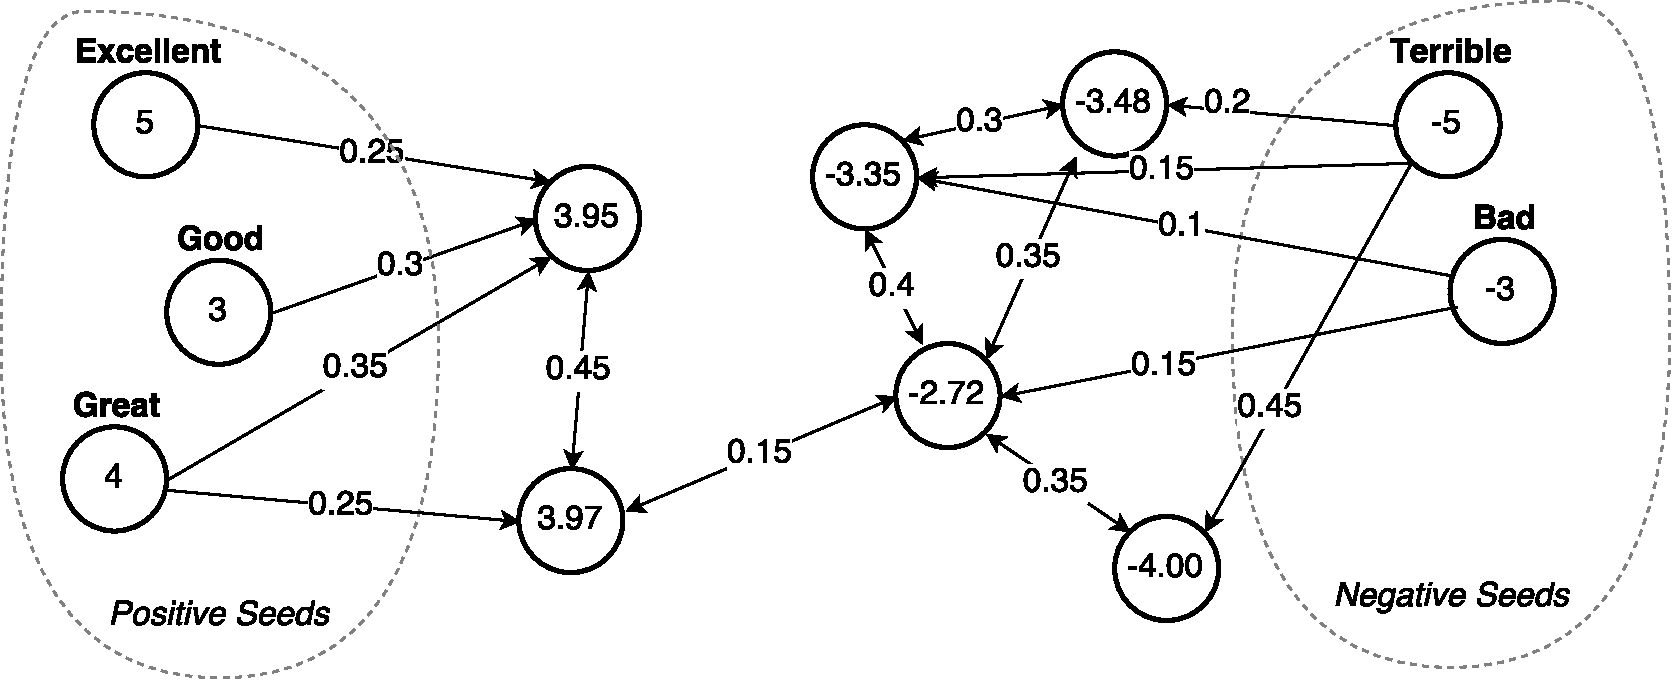
\includegraphics[width=\textwidth]{./figs/label_propagation}
        \caption{Using the Label Propagation Algorithm}
        \label{fig:label_propagation}
    \end{subfigure}
    \begin{subfigure}[b]{1.0\textwidth}
        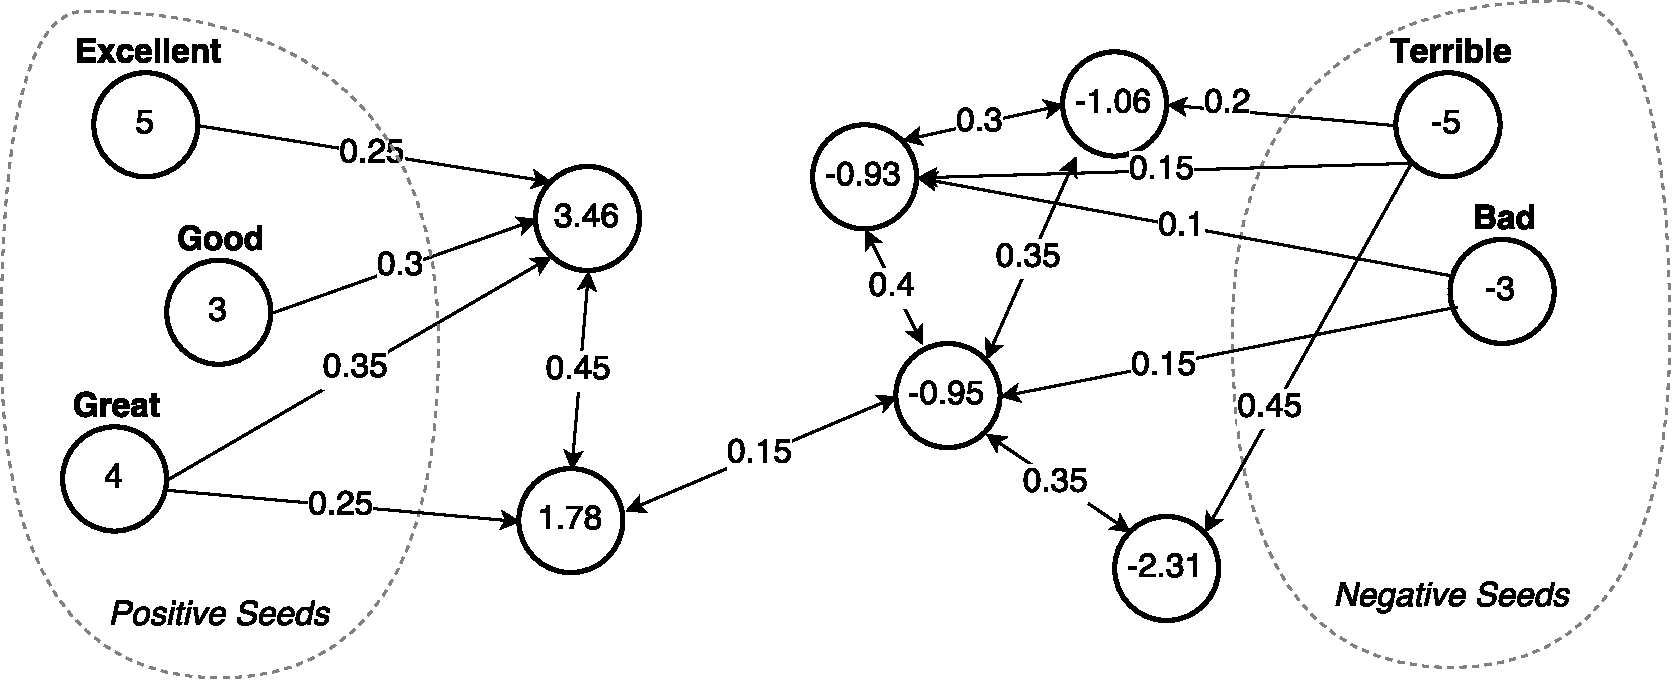
\includegraphics[width=\textwidth]{./figs/graph_propagation}
        \caption{Using the Graph Propagation Algorithm}
        \label{fig:graph_propagation}
    \end{subfigure}
    \caption{Comparison of propagation algorithms' end results}
    \label{fig:propagation_comparison}
\end{figure}


\subsection{Graph Propagation Algorithm}
\label{sec:graph_propagation_algorithm}
The Graph Propagation Algorithm is an alternate version of the LPA, specifically aimed towards sentiment lexicon creation based on graphs of lower quality, where not all edges are trustworthy. The algorithm was proposed by \cite{Velikovich2010}, arguing that the approach would alleviate the reinforcement effect of the LPA on lower quality graphs. Similarly to the LPA, an initial graph is created based on an appropriate relationship measure before all nodes representing the seed words are given an initial sentiment value. The nodes representing seed words are then traversed, propagating their sentiment value to all nodes within a distance $T$. On each step away from the seed node, the sentiment value is weighted using the edge weights between the nodes, representing their relational strength. The further away from the seed node a node is located, the lower the propagated sentiment value will be. Each node holds the max path from each seed node within a distance of $T$. After all seed nodes have propagated their sentiment value, the final sentiment value of each node is calculated by subtracting the sum of the max paths from negative seed nodes from the sum of max paths from positive seed nodes. The method is shown in Algorithm~\ref{alg:graph_propagation}. \\

\begin{algorithm}[t]
	\DontPrintSemicolon
    \caption{Graph Propagation Algorithm}
    \label{alg:graph_propagation}
    \KwIn{$G=(V,E)$, $w_{ij}\in[0,1]$, $\gamma \in \mathbb{R}$, $T\in \mathbb{N}$, $P$, $N$}
    \KwOut{Sentiment Lexicon, $pol \in \mathbb{R}^{|V|}$}
    
    $pol_i, pol_i^+, pol_i^- = 0$, $\forall i$\;
	$pol_i^+ = 1.0$, $\forall v_i \in P$\;
    $pol_i^- = 1.0$, $\forall v_i \in N$\;

	$a_{ii} = 1, a_{ij} = 0$, $\forall i \neq j$\;

	\For{$v_i \in P$}{
    	$F=\{v_i\}$\;
        \For{$t \gets 1$ \textbf{to} $T$}{
        	\For{$(v_k, v_j) \in E$ such that $v_k \in F$}{
            	$a_{ij} = \max \{a_{ij}, a_{ik} \cdot w_{kj}$\}\;
                $F=F \bigcup \{v_j\}$
        	}
        }
    }
    \For{$v_j \in V$}{
    	$pol_j^+ = \sum_{v_i \in P} a_{ij}$
    }

	Repeat steps 4-12 using $N$ to compute $pol^-$\;

	$\beta = \sum_i pol_i^+ / \sum_i pol_i^-$\;
	$pol_i = pol_i^+ - \beta pol_i^-$, $\forall i$\;
	\textbf{if} $|pol_i| < \gamma$ \textbf{then} $pol_i=0.0$, $\forall i$\;
\end{algorithm}

Figure~\ref{fig:graph_propagation} shows the result of running the Graph Propagation Algorithm on a small, dense graph. Notice how using LPA, a node received higher sentiment value having only one edge from positive seed words than a node having three edges from positive seed words, whereas using the Graph Propagation Algorithm, the more connected node received a much higher sentiment value than the single connected node.


\section{Classification Scoring Metrics}
\label{sec:classification_scoring_metrics}
To measure the performance of a classification system, a collection of scoring metrics are needed. In Sentiment Analysis the four scoring metrics precision, recall, F1--score and accuracy are often used. The calculation of these depends on values called \textit{true-positives}, \textit{false-positives}, \textit{true-negatives} and \textit{false-negatives}; $tp$, $fp$, $tn$ and $fn$ respectively. Here $tp$ and $tn$ are the number of examples correctly classified as positive and negative, while $fp$ and $fn$ are the number of examples falsely classified as positive and negative. This relationship can be viewed in the confusion matrix displayed in Table~\ref{tab:prediction_outcomes}.

\begin{table}[H]
    \centering
    \begin{tabular}{l|l|c|c|c}
        \multicolumn{2}{c}{}&\multicolumn{2}{c}{Predicted}&\\
        \cline{3-4}
        \multicolumn{2}{c|}{} & Positive & Negative\\
        \cline{2-4}
        \multirow{2}{*}{\rot{True}} & Positive & $tp$ & $fn$\\
        \cline{2-4}
        & Negative & $fp$ & $tn$\\
        \cline{2-4}
    \end{tabular}
    \caption{Confusion matrix for possible prediction outcomes}
    \label{tab:prediction_outcomes}   
\end{table}

\subsection*{Precision}
Precision is the ratio of the number of relevant returned results to the number of total returned results. The precision ratio describes how many of the returned results are relevant. Precision is defined as:
\begin{equation*}
    precision = \frac{tp}{tp+fp}
\end{equation*}

\subsection*{Recall}
Recall is the ratio of the number of relevant results to the number of overall relevant results. The recall ratio describes how many of the relevant results are returned.  Recall is defined as:
\begin{equation*}
    recall = \frac{tp}{tp+fn}
\end{equation*}

\subsection*{$F_{1}$-Score}
F-Score is the weighted combination of precision and recall, and in its general form defined as:
\begin{equation*}
    F_{\beta} = (1+\beta)\cdot\frac{precision\cdot recall}{(\beta ^2 \cdot precision) + recall}
\end{equation*}

The most commonly used $\beta$ value is $1$, this is known as $F_{1}$-score, which produces the harmonic mean of precision and recall. $F_{1}$-score is thus defined as:
\begin{equation*}
    F_{1} = 2\cdot\frac{precision\cdot recall}{precision + recall} = \frac{2tp}{2tp + fp + fn}
\end{equation*}

\subsection*{Accuracy}
Accuracy is the ratio of the number of true results to the number of total cases. The accuracy ratio describes how many of the results were accurately predicted as positive and negative. Accuracy is defined as:
\begin{equation*}
    accuracy = \frac{tp+tn}{tp+fp+tn+fn}
\end{equation*}


\section{Tools}
\label{sec:tools}

\subsection{Scikit-Learn}
\label{sec:background_scikit}
Scikit-Learn, by \cite{scikit-learn}, is a machine learning library, written in Python. It consists of implementations of a wide range of state-of-the-art machine learning algorithms built for both supervised and unsupervised medium-scale problems. It emphasises ease of use and good documentation, and plays an important role in this project. In the following paragraphs the most relevant concepts and features of Scikit-Learn are presented.

\subsection*{Transformer}
A \textit{Transformer} object in Scikit-Learn is used to extract or generate feature representations of the data. To extract different features, different transformers must be created.

\subsection*{Pipeline}
Scikit-Learn provides a \textit{Pipeline} object, allowing pipelining of machine learning processes. The pipeline makes it easy to perform and chain processes such as preprocessing and feature extraction together with a machine learning algorithm in a sequential and tidy manner. In other words, it allows sequential and parallel application of a list of estimators. An estimator is in this context either an object that is able to learn from data, such as a classifier, or a \textit{Transformer} object that extracts features from raw data.

\subsection*{Feature Union}
A \textit{Feature Union} is an object included in the \textit{Pipeline} framework and is a useful tool in feature extraction. The standard \textit{Pipeline} chains transformers together in a sequential manner where data from one \textit{Transformer} is fed directly into the next \textit{Transformer}. A \textit{Feature Union} on the other hand allows for a collection of transformers to be fed the exact same input data. This is especially useful when wanting to extract a series of different features from the same data. The resulting feature vectors from the \textit{Transformer}s in the \textit{Feature Union} are concatenated into a final feature matrix. 

\subsection*{Grid Search}
The \textit{Pipeline} framework allows performing a \textit{Grid Search} across all \textit{Transformer} or estimator parameters. The \textit{Grid Search} takes a set of possible values for each parameter in each transformer and searches through all possible parameter combinations, looking for the combination that yields the best performance overall.

\subsection{GATE TwitieTagger}
The GATE TwitieTagger, by \cite{twitieTagger}, is a \acf{pos} tagger specifically created for tweets. As described in Section~\ref{sec:background_nlp}, the \ac{pos} tagger takes as input a sentence and returns the same sentence where each word is replaced by its \ac{pos} tag. \\

Another powerful \ac{pos} tagger tailored for tweets is the TweeboParser by \cite{Gimpel11}. TweeboParser is very complex and is written in several programming languages linked together with Shell and Python scripts. Because of this, we decided to use the much simpler GATE TwitieTagger which is only written in Java. In terms of performance, both report a similarly high token accuracy values: 91\% and 90\% for GATE TwitieTagger and TweeboParser, respectively.

\subsection{VADER Sentiment Analysis}
\label{sec:vaderSentiment}
VADER (Valence Aware Dictionary and sEntiment Reasoner), by \cite{vaderSentiment}, is a lexicon based sentiment analysis tool specifically tuned towards social media. VADER goes beyond the simple bag-of-words model and takes into consideration word order and degree modifiers.

\subsection{Emoji-Java}
Emoji-Java\footnote{Emoji-Java: \url{https://github.com/vdurmont/emoji-java}} is a lightweight library that lets you convert from Unicode emoji characters to their alphabetical, decimal and hexadecimal representations. The alphabetical representation, called alias, is a single word describing emote; for example, {\DejaSans ☺} is translated into "smile".


\section{Datasets}
\label{sec:datasets}
In this section all external datasets used is described. In addition we downloaded a large Twitter dataset using the Tweet Streaming API to create our sentiment lexicon. That dataset is described in detail in Section~\ref{sec:twitter_streaming_dataset}.

\subsection{TweetNLP --- Twitter Word Cluster}
\label{sec:tweetnlp}
TweetNLP is a set of tools made specifically for Twitter \ac{nlp} tasks. A part of TweetNLP is a hierarchical Twitter word cluster, by \cite{Owoputi12}, that was generated using Brown clustering, based on 56 million unique tweets. We have incorporated this clustering as a simple dictionary from word to cluster ID. 

\subsection{SemEval 2016 Twitter Sentiment Dataset}
As part of the \ac{semeval} 2016 five datasets have been made available. These comprise a training set and a test set from \ac{semeval} 2013, and test sets from \ac{semeval} 2014, 2015 and 2016. We used the 2013 training sets for training, while the test sets were only used to test our system. To access the datasets, they all had to be downloaded through the Twitter API. Portions of the tweets have been deleted since the datasets were originally created and are therefore no longer available. Table~\ref{tab:dataset_overview} gives an overview of the datasets used, comparing the sizes of the original annotated datasets to the sizes and class distributions of the datasets actually available at the time they were downloaded.

\makeatletter
    \setlength\@fptop{0\p@}
\makeatother

\begin{table}[htbp]
    \begin{tabular}{| l | l | l | l | l | l |}
        \hline
         & \multicolumn{2}{c|}{\textbf{Size}} & \multicolumn{3}{c|}{\textbf{Class distribution}} \\ \hline
        \textbf{Name} & \textbf{Original} & \textbf{Downloaded} & \textbf{Positive} & \textbf{Neutral} & \textbf{Negative} \\ \hline
        2013-train & 9684 & 8748 & 3283 & 4175 & 1290 \\ \hline
        2013-test & 3813 & 3087 & 1258 & 1367 & 462 \\ \hline
        2014-test & 1853 & 1509 & 794 & 564 & 151 \\ \hline
        2015-test & ? & 2390 & 1038 & 987 & 365 \\ \hline
        2016-test & ? & 20632 & 7059 & 10342 & 3231 \\ \hline
    \end{tabular}
    \caption{Overview of SemEval datasets used in the project}
    \label{tab:dataset_overview}
\end{table}

\glsresetall
